\chapter{Présentation d'E-protect}

\section{Contexte}

\subsection*{Progression du nombre de cambriolages en France}

Selon l'Observatoire national de la délinquance et de la réponse pénale (ONDRP), le nombre des vols commis aux domiciles des particuliers et dans les entrepôts a une nouvelle fois augmenté en 2013, de $7.2\%$ en zone urbaine sur un an.

2013: hausse de $6.4\%$ (par rapport à 2012) des cambriolages en zone urbaine et de $4.7\%$ en zone rurale. Les cambriolages dans les habitations principales ont respectivement augmenté, dans ces mêmes zones, de $7\%$ et de $1.3\%$ et ceux des résidences secondaires de $10\%$ et $17.7\%$.

Les cambriolages de résidences principales ont bondi de $11.3\%$ en 2014 dans les secteurs ruraux et périurbains. Soit, $23300$ cambriolages de plus en 12 mois!\\

Il se produit un cambriolage toutes les $1.5$ minutes en France, soit près de $985$ cambriolages par jour($323000$ en 2011 et $359500$ en 2012) ; Dopant le business des alarmes et des portes blindées. Le nombre de cambriolages est en hausse constante : sur les 6 prochaines années un Français a 1 chance sur 10 de se faire cambrioler, tout en sachant que cette statistique ne tient pas compte des tentatives ou cambriolages non déclarés.\\

\subsection*{Les chiffres clés}
\begin{itemize}
	\item $8\%$ des foyers français étaient équipés d'une porte blindée en France en 2009
	\item $95\%$ des cambrioleurs prennent la fuite en cas de déclenchement d’une alarme. Un argument majeur pour s'équiper !
	\item Les cambriolages représentent $14\%$ des atteintes aux biens.
	\item $80\%$ des cambriolages ont lieu en ville et $13\%$ seulement sont élucidés.
	\item $50\%$ des cambriolages concernent les résidences principales, $6\%$ les résidences secondaires et $44\%$ les locaux professionnels.
	\item $80\%$ des cambrioleurs empruntent la porte, les autres passent par le toit ou les fenêtres.
	\item 5 minutes : c'est le délai moyen après lequel le monte-en-l'air abandonne son effraction.
	\item En général, un cambriolage ne dépasse pas une vingtaine de minutes.
	\item $22\%$ des Français ayant subi un cambriolage n'ont absolument rien fait par la suite pour améliorer leur sécurité !
	\item $80\%$ des cambriolages ont lieu en plein jour, $55\%$ entre 14 et 17H
	\item Il y a donc également $20\%$ des cambriolages la nuit pendant le sommeil des propriétaires
	\item $6500$\euro : Un cambriolage dans une résidence principale coûte à ses victimes près de $6500$ euros.\\
\end{itemize}

\subsection*{Récapitulatif}
\begin{itemize}
	\item $382000$ en 2013 : $+6\%$
	\item $359500$ en 2012 : $+11\%$
	\item $323000$ en 2011\\
\end{itemize}


\begin{figure}[h!]
	\begin{center}
		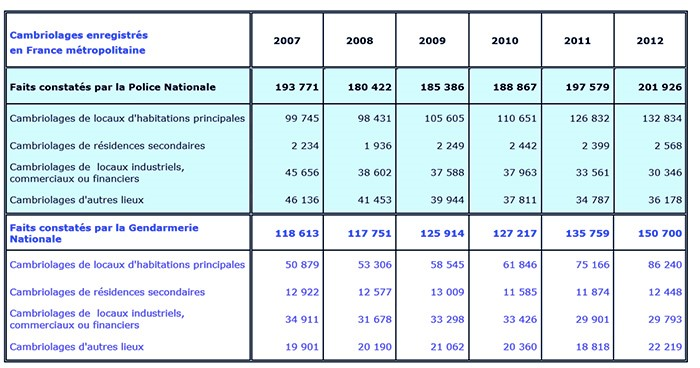
\includegraphics[width=0.98\linewidth]{imgs/vols_france}
	\end{center}
	\caption{Cambriolages enregistrés par la police nationale (zone urbaine) ou par la gendarmerie nationale (zone rurale) en France de 2007 à 2012 \cite{www:DCpj}}
\end{figure}

En tête du classement on trouve la Guadeloupe. Avec un taux de $6.5$ cambriolages pour $1000$ habitants, elle précède le Vaucluse ($6.4$ pour $1000$ habitants). De manière générale, les départements d’outre-mer sont parmi les plus exposés au risque de cambriolage. La Guyane affiche ainsi une statistique de $6$ pour $1000$ habitants. Concernant le France métropolitaine, le sud-est est particulièrement touché par les affaires de cambriolages d’habitations principales.\\

Six départements ont un taux compris entre $5.4$ et $6.5$ pour $1000$ habitants (les Pyrénées-Orientales, l’Hérault, le Gard, le Vaucluse, les Bouches du Rhône et les Alpes-Maritimes).\\

L’Île de France que l’on pourrait considérer comme une région très exposée limite la casse et reste dans la moyenne nationale de $2.7/1000$ habitants. A l’inverse, le risque de se faire cambrioler est extrêmement faible dans le centre de la France. Les résidents du Cantal peuvent dormir sur leurs deux oreilles avec seulement $0.3$ cambriolage pour $1000$ habitants département du Cantal. La Haute-Corse connaît la plus forte variation à la hausse avec une augmentation de $71.4\%$.\\

L'importance de développer des solutions de protections est bien réelle. De nos jours lorsque l'on achète une alarme pour notre domicile, il faut obligatoirement avoir l'aide d'un technicien pour la poser. Si l'on souhaite installer d'autres capteurs, il faut rappeler un technicien (perte de temps, et obligation de se libérer pour être présent). Du point de vue du client, cela est contraignant car il dépend d'un organisme extérieur. De plus, le fait de faire installer l'alarme par une personne inconnue est un risque potentiel.\cite{www:ONDRP}\\


\section{Objet du projet}

L'importance de développer des solutions de protections est bien réelle.\\
La procédure actuelle mobilise beaucoup de temps et représente un investissement financier certain du point de vue client. L’installation ou modifications de système d’alarmes nécessite obligatoirement l’intervention d’un technicien, facturé, dans une plage horaire poussant le client à se libérer de ses activités professionnelles.\\

E-protect libère des ces contraintes, proposant un produit modulable et installable directement par le client, bénéficiant d’un service de conseils gratuit, celui-ci n’a plus à dépendre d’un organisme extérieur.\\

Le produit proposé est un système d’alarme résidentiel connecté, facile à installer et à configurer. Afin de proposer un système le moins chère possible, E-protect s’appuie sur l’élimination des intermédiaires et utilise un réseau meshe de capteurs intelligent, travaillant sur une portée moins importante et jouant ainsi sur la connexion des capteurs entre eux. L'installation des composants du système E-protect est beaucoup plus simple qu'un système d'alarme filé. Nul besoin de percer les murs et de poser des conducteurs, ce qui réduit considérablement les frais d'installation.\\

Accessible depuis internet et une application Smartphone, E-protect assure un contact permanent entre le client et le domicile.\\

Le système E-protect comporte aussi :
\begin{itemize}
	\item Une connexion avec le poste de police le plus proche;
	\item Un système Backup en cas de défaillance du réseau électrique;
	\item Un design de capteur innovant et modulable selon la volonté du client;
	\item Une consommation énergétique très faible, reposant sur un appel de puissance réduit du fait de l’utilisation d’un réseau meshe.
\end{itemize}